\documentclass[11pt, twoside]{report}

\usepackage{fontspec}
\usepackage[utf8]{inputenc}
\usepackage[bitstream-charter]{mathdesign}
\usepackage{bbding}
\usepackage{ragged2e}
\usepackage{parskip}
\usepackage{enumitem}
\usepackage{titlesec}
\usepackage{paracol}
\usepackage{mdframed}
\usepackage[margin=1in]{geometry}

\usepackage[autocompile]{gregoriotex}

\titleformat{\chapter}[block]{\huge\scshape\filcenter}{}{1em}{}
\titleformat{\section}[block]{\Large\bfseries\filcenter}{}{1em}{}

\mdfsetup{skipabove=\topskip, skipbelow=\topskip}

\newcommand{\rubric}[1]{
	\switchcolumn[0] {
		\itshape
		#1
	}
}

\newcommand{\latinenglish}[2]{
	\switchcolumn[0]* {
		#1
	}
	\switchcolumn[1] {
		\itshape\small
		#2
	}
}

\newcommand{\latinenglishequal}[2]{
	\switchcolumn[0]* {
		#1
	}
	\switchcolumn[1] {
		\itshape
		#2
	}
}

\newenvironment{latinenglishsection}
	{\columnratio{.7, .3} \begin{paracol}{2}}
	{\end{paracol}}

\newenvironment{latinenglishequalsection}
	{\columnratio{.5, .5}\begin{paracol}{2}}
	{\end{paracol}}

\setlength{\columnseprule}{0.4pt}

\newcommand{\heading}[1]{
	\begin{leftcolumn}
		#1
	\end{leftcolumn}
}

\newcommand{\spanning}[1]{
	\switchcolumn*[#1]
}

\newenvironment{verses}[1]
	{\begin{flushleft} \begin{enumerate}[leftmargin=*] \setcounter{enumi}{#1}}
	{\end{enumerate} \end{flushleft}}

\newenvironment{versicles}{\par\leavevmode\parskip=0pt}{}

\newenvironment{collect}
{
	\leavevmode
	\parindent=1em
	\parskip=0pt
	\noindent Orémus.\par
}{}

\newenvironment{optionbox}
{
	\switchcolumn[0]
	\begin{mdframed}
%	\begin{minipage}{0.8\linewidth}
}{
%	\end{minipage}
	\end{mdframed}
}

\newcommand{\optionrule}{
	\begin{center}
	\rule{0.5\linewidth}{0.6pt}
	\end{center}
}

\newenvironment{optionruled}
{
	\optionrule
}
{
	\optionrule
}

% for use inside the collect environment
\newcommand{\Amen}{\par\noindent \Rbar. Amen.}

\begin{document}

\vspace*{4cm}

\begin{center}
	\textbf{\Huge Prime of the Blessed Virgin Mary}\\
	{\LARGE According to the Washtenaw Use}
\end{center}

\vspace*{1cm}
%\maketitle

%\begin{figure}[h!]
	%\centering
%\end{figure}

\begin{center}
	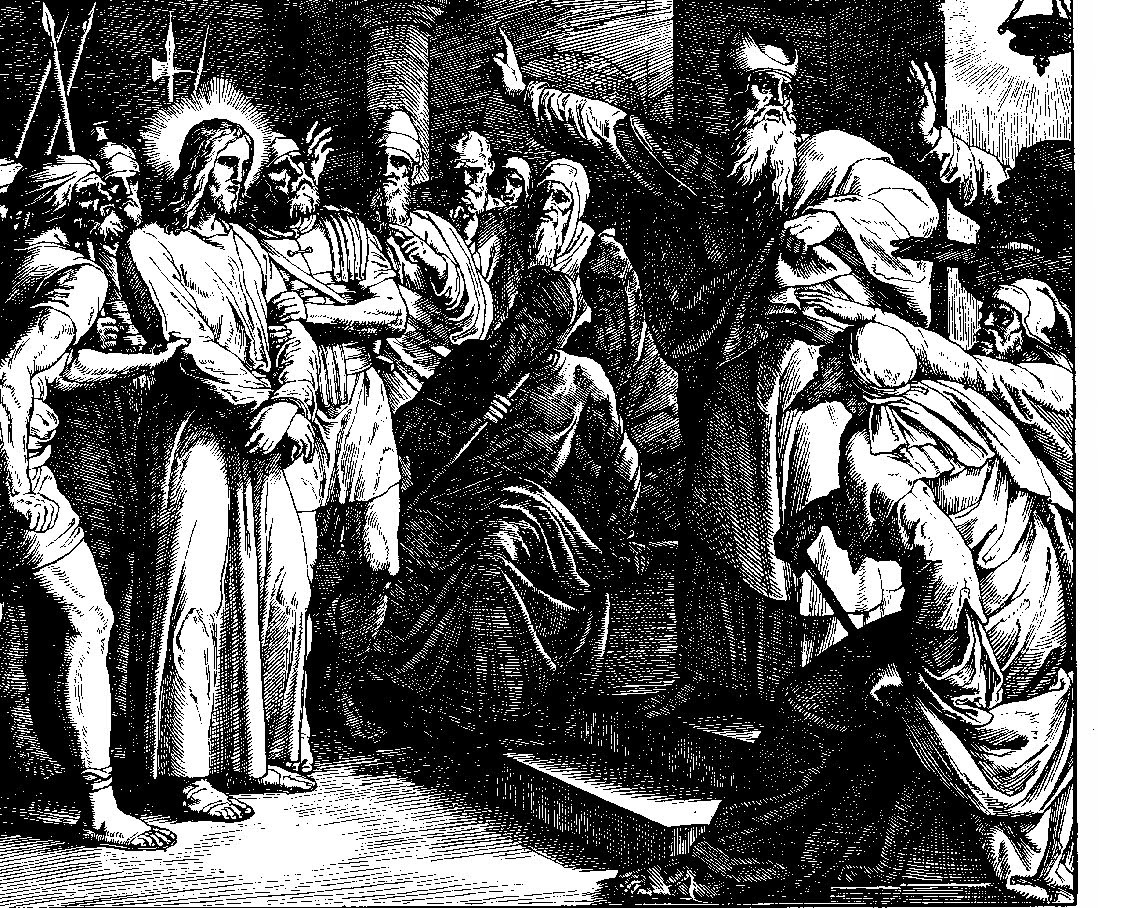
\includegraphics[width=\textwidth]{ChristAccused}
\end{center}

\hspace{0pt}
\vfill

\pagebreak

\vspace*{7.5cm}
``At \textit{Prime} tide Our Lord Jesus Christ was led to Pilate, and accused; in the same hour after His Resurrection, He appeared to Mary Magdalen, and another day He appeared to His disciples as they were fishingm at the same hour... At the time of \textit{Prime}, there appeareth a star before the sun, as if it were the ladder or bringer forth of the sun; and Our Lady came before and brought forth to mankind that Sun of Righteousness that is Our Lord Jesus Christ.'' (Paraphrased from the \textit{Mirror of Our Lady}.) O Most Blessed Virgin, who brought forth the Sun of Righteousness, pray for us that we too may see and know Our Risen Lord. Amen.
\vfill

\pagebreak

\chapter*{Before Prime}

\section*{Preparatory Prayers}

\textit{All kneel and pray silently. As you say the prayer \textnormal{Aperi, Domine}, make the sign of the cross with your thumb first over your lips, and then over your heart.}

\begin{latinenglishequalsection}

\latinenglishequal{
	Áperi, {\color{red}\maltese}\ Dómine, os meum ad benedicéndum\linebreak nomen sanctum tuum:
	{\color{red}\maltese}\ munda quoque cor meum ab ómnibus vanis, pervérsis et aliénis cogitatiónibus;
	intelléctum illúmina, afféctum inflámma, ut digne, atténte ac devóte hoc Offícium beátæ Vírginis Maríæ recitáre váleam,
	et exaudíri mérear ante conspéctum divínæ Majestátis tuæ.
	Per Christum Dóminum nostrum. 
	Amen.
}{
	Open, {\color{red}\maltese}\ O Lord, my mouth to bless Thy holy Name; {\color{red}\maltese}\ cleanse also my heart from all vain, evil, and wandering thoughts; enlighten my understanding and kindle my affections; that I may worthily, attentively, and devoutly say this Office of the Blessed Virgin Mary, and so merit to be heard before the presence of Thy divine Majesty.  Through Christ our Lord.  Amen.
}

\latinenglishequal{
	Domine, in unióne illíus divínæ intentiónis, qua ipse in terris laudes Deo persolvísti, has tibi Horas persólvo.
}{
	O Lord, in union with that divine intention wherewith thou, whilst here on earth, didst render praises unto God, I desire to offer this my Office of prayer unto thee.
}

\latinenglishequal{
	Ave María, grátia plena, Dóminus tecum. Benedíc\-ta tu in muliéribus, et benedíctus fructus ventris tui, Jesus.
 Sancta María, Mater Dei, ora pro nobis peccatóribus, nunc et in hora mortis nostræ. Amen.
 }{
 	Hail Mary, full of grace, the Lord is with thee. Blessed art thou among women, and blessed is the fruit of thy womb, Jesus.
 Holy Mary, Mother of God, pray for us sinners, now and at the hour of our death. Amen.
 }
 
 \end{latinenglishequalsection}
 
\chapter*{Prime}

\begin{latinenglishsection}

\heading{\section*{Invitatory}}

\rubric{\color{red}All make the Sign of the Cross as the Officiant says the ``Deus in Adjutorium''. All continue together with the entire ``Gloria Patri'' after the response: }

\latinenglish{
	\gresetinitiallines{1}
	\gregorioscore{deus_in_adjutorium_minor}
}{
	O God, come to my assistance.
		
	O Lord, make haste to help me.
	
	Glory be to the Father, and to the Son, and to the Holy Spirit,
	as it was in the beginning, is now, and ever shall be, world without end. Amen.
	
	Alleluia.
}

\rubric{\color{red}From Septuagesima until Easter, \textnormal{Alleluia} is replaced with:}

\latinenglish{
	\gresetinitiallines{0}
	\gabcsnippet{
	(c3)Lau(h)s ti(h)bi(h) Dó(h)mi(h)ne(h), Re(h)x æ(h)té(h)rnæ(i) gló(h)ri(h)æ.(g) (::)
	}
}{
	Praise to thee, O Lord, King of everlasting glory.
}

\end{latinenglishsection}

\vfill\pagebreak

\begin{latinenglishsection}

\heading{\section*{Hymn}}

\latinenglish{
	\gresetinitiallines{0}
	\gregorioscore{memento_rerum_conditor}
}{
	1. Remember, Maker of all things,
	That once the form of our flesh, 
	From the Virgin's sacred womb, 
	Being born, Thou didst assume.
	
	2. Mary, Mother of grace, 
	Sweet parent of clemency, 
	Thou protect us from the enemy, 
	And receive us at the hour of death.
	
	3. Jesus, to Thee be glory, 
	Who wast born of the Virgin, 
	With the Father, and the loving Spirit, 
	Unto sempiternal ages. Amen.
}

\rubric{\color{red} For `Throughout the Year', \underline{see page 6}.}
\rubric{\color{red} For `Advent', \underline{see page 9}.}
\rubric{\color{red} For `Christmastide', \underline{see page 12}.}

\end{latinenglishsection}

\vfill\pagebreak

\section*{THROUGHOUT THE YEAR}

\begin{latinenglishsection}

\heading{\section*{Psalm 53}}

\rubric{\color{red}The Cantor intones the antiphon and leads the first Psalm verse to the star (*). All sit, while the Cantor's side finishes the first verse together. The Officiants side then says the second Psalm verse, with each side alternating thereafter. The remaining Psalms are intoned up to the asterisk by the Cantor, repeating the pattern of sitting and standing until the antiphon is said in full at the very end.}

\latinenglish{
	\gresetinitiallines{1}
	\gregorioscore{assumpta_est_intonation}
}{
	Mary was taken up...
}

\latinenglish{
	\gresetinitiallines{0}
	\gregorioscore{psalm_53_1_7a}
	
	\begin{verses}{1}
	
	\item Deus, exáudi orati\textbf{ó}nem \textbf{me}am:~* áuribus pércipe verba \textbf{o}ris \textbf{me}i.

	\item Quóniam aliéni insurrexérunt advérsum me,~{\color{red}\GreDagger}\  et fortes quæsiérunt \textbf{á}nimam \textbf{me}am:~* et non proposuérunt Deum ante con\textbf{spéc}tum \textbf{su}um.
	
	\item Ecce enim Deus \textbf{ád}ju\textbf{vat} me:~* et Dóminus suscéptor est \textbf{á}nimæ \textbf{me}æ.
	
	\item Avérte mala ini\textbf{mí}cis \textbf{me}is:~* et in veritáte tua dis\textbf{pér}de \textbf{il}los.
	
	\item Voluntárie sacrifi\textbf{cá}bo \textbf{ti}bi,~* et confitébor nómini tuo, Dómine: \textbf{quón}iam \textbf{bo}num est:
	
	\item Quóniam ex omni tribulatióne e\textbf{ri}pu\textbf{ís}ti me:~* {\color{red}\textit{(stand)}} et super inimícos meos despéxit \textbf{ó}culus \textbf{me}us.
	
	\item {\color{red}\textit{(bow)}} Glória \textbf{Pa}tri, et \textbf{Fí}lio,~* et Spi\textbf{rí}tui \textbf{Sanc}to.
	
	\item {\color{red}\textit{(rise)}} Sicut erat in princípio, et \textbf{nunc}, et \textbf{sem}per,~* et in s\'{\ae}cula sæcu\textbf{ló}rum. \textbf{A}men.
	
	\end{verses}
}{
	1. O God, save me in thy name:
	and judge me in thy strength.
	
	2. O Lord, hear my prayer:
	and hearken to the words of my mouth.
	
	3. For strangers have risen up against me, and the mighty have sought after my soul:
	and they have not set God before their eyes.
	
	4. Behold, God is my helper:
	and the Lord upholdeth my soul.
	
	5. Turn back the evil upon mine enemies:
	and destroy them in thy truth.
	
	6. Freely will I sacrifice unto thee:
	and will praise thy name, O Lord, for it is good.
	
	7. For thou hast delivered me out of all trouble:
	and mine eye hath looked down upon mine enemies.
	
	8. Glory be to the Father, and to the Son, and to the Holy Spirit:
	As it was in the beginning, is now, and ever shall be, world without end. Amen.
}

\end{latinenglishsection}

\vfill\pagebreak

\begin{latinenglishsection}

\heading{\section*{Psalm 84}}

\latinenglish{
	\gresetinitiallines{0}
	\gregorioscore{psalm_84_1_7a}
	
	\begin{verses}{1}
	
	\item Remisísti iniquitátem \textbf{ple}bis \textbf{tu}æ:~* operuísti ómnia pec\textbf{cá}ta e\textbf{ó}rum.

	\item Mitigásti omnem \textbf{i}ram \textbf{tu}am:~* avertísti ab ira indignati\textbf{ó}nis \textbf{tu}æ.
	
	\item Convérte nos, Deus, salu\textbf{tá}ris \textbf{nos}ter:~* et avérte iram \textbf{tu}am a \textbf{no}bis.
	
	\item Numquid in ætérnum ira\textbf{scé}ris \textbf{no}bis?~* aut exténdes iram tuam a generatióne in gene\textbf{ra}ti\textbf{ó}nem?
	
	\item Deus, tu convérsus vi\textbf{vi}fi\textbf{cá}bis nos:~* et plebs tua læ\textbf{tá}bitur \textbf{in} te.
	
	\item Osténde nobis, Dómine, miseri\textbf{cór}diam \textbf{tu}am:~* et salutáre \textbf{tu}um da \textbf{no}bis.
	
	\item Audiam quid loquátur in me \textbf{Dó}minus \textbf{De}us:~* quóniam loquétur pacem in \textbf{ple}bem \textbf{su}am.
	
	\item Et super \textbf{sanc}tos \textbf{su}os:~* et in eos, qui conver\textbf{tún}tur \textbf{ad} cor.
	
	\item Verúmtamen prope timéntes eum salu\textbf{tá}re ip\textbf{sí}us:~* ut inhábitet glória in \textbf{ter}ra \textbf{nos}tra.
	
	\item Misericórdia, et véritas obvia\textbf{vé}runt \textbf{si}bi:~* justítia, et pax \textbf{os}cu\textbf{lá}tæ sunt.
	
	\item Véritas de \textbf{ter}ra \textbf{or}ta est:~* et justítia de \textbf{cæ}lo pro\textbf{spé}xit.
	
	\item Etenim Dóminus dabit be\textbf{ni}gni\textbf{tá}tem:~* et terra nostra dabit \textbf{fruc}tum \textbf{su}um.
	
	\item Justítia ante eum \textbf{am}bu\textbf{lá}bit:~* {\color{red}\textit{(stand)}} et ponet in via \textbf{gres}sus \textbf{su}os.
	
	\item {\color{red}\textit{(bow)}} Glória \textbf{Pa}tri, et \textbf{Fí}lio,~* et Spi\textbf{rí}tui \textbf{Sanc}to.
	
	\item {\color{red}\textit{(rise)}} Sicut erat in princípio, et \textbf{nunc}, et \textbf{sem}per,~* et in s\'{\ae}cula sæcu\textbf{ló}rum. \textbf{A}men.
	
	\end{verses}
}{
	1. Thou hast blessed thy land, O Lord:
	thou hast turned away the captivity of Jacob.
	
	2. Thou hast forgiven the iniquity of thy people:
	thou hast covered all their sins.
	
	3. Thou hast softened all thine anger:
	thou hast turned thyself from thy wrathful indignation.
	
	4. Convert thou us, O God our Saviour:
	and turn away thine anger from us.
	
	5. Wilt thou be angry with us forever:
	or wilt thou stretch out thy wrath from generation to generation?
	
	6. Thou wilt turn again, O God, and quicken us:
	and thy people shall rejoice in thee.
	
	7. Shew us, O Lord, thy mercy:
	and grant us thy salvation.
	
	8. I will hearken what the Lord God shall say within me:
	for he will speak peace unto his people:
	
	9. Unto his Saints likewise:
	and to those who are converted in heart.
	
	10. Surely his salvation is nigh unto them that fear him:
	that glory may dwell in our land.
	
	11. Mercy and truth have met together:
	justice and peace have kissed each other.
	
	12. Truth is sprung out of the earth:
	and justice hath looked down from heaven.
	
	13. For the Lord shall put forth his goodness:
	and our land shall yield her fruit.
	
	14. Justice shall walk before him: 
	and shall set his footsteps in the way.
	
	15. Glory be to the Father, and to the Son, and to the Holy Spirit:
	As it was in the beginning, is now, and ever shall be, world without end. Amen.
}

\end{latinenglishsection}

%\vfill\pagebreak

\begin{latinenglishsection}

\heading{\section*{Psalm 116}}

\latinenglish{
	\gresetinitiallines{0}
	\gregorioscore{psalm_116_1_7a}
	
	\begin{verses}{1}
	
	\item Quóniam confirmáta est super nos miseri\textbf{cór}dia \textbf{e}jus:~* {\color{red}\textit{(stand)}} et véritas Dómini manet \textbf{in} æ\textbf{tér}num.

	\item {\color{red}\textit{(bow)}} Glória \textbf{Pa}tri, et \textbf{Fí}lio,~* et Spi\textbf{rí}tui \textbf{Sanc}to.
	
	\item {\color{red}\textit{(rise)}} Sicut erat in princípio, et \textbf{nunc}, et \textbf{sem}per,~* et in s\'{\ae}cula sæcu\textbf{ló}rum. \textbf{A}men.
	
	\end{verses}
	
	\gresetinitiallines{1}
	\gregorioscore{assumpta_est}
}{
	1. Praise the Lord, all ye gentiles:
	praise him, all ye people.
	
	2. For his mercy is confirmed upon us:
	and the truth of the Lord endureth forever.
	
	3. Glory be to the Father, and to the Son, and to the Holy Spirit:
	As it was in the beginning, is now, and ever shall be, world without end. Amen.
	
	Mary was taken up to heaven: the angels rejoice, and with praises bless the Lord.
}

\rubric{\color{red}Proceed to page 15.}

\end{latinenglishsection}

\vfill\pagebreak

\section*{ADVENT}

\begin{latinenglishsection}

\heading{\section*{Psalm 53}}

\rubric{\color{red}The Cantor intones the antiphon and leads the first Psalm verse to the star (*). All sit, while the Cantor's side finishes the first verse together. The Officiants side then says the second Psalm verse, with each side alternating thereafter. The remaining Psalms are intoned up to the asterisk by the Cantor, repeating the pattern of sitting and standing until the antiphon is said in full at the very end.}

\latinenglish{
	\gresetinitiallines{1}
	\gregorioscore{missus_est_intonation}
}{
	The Angel Gabriel was sent...
}

\latinenglish{
	\gresetinitiallines{0}
	\gregorioscore{psalm_53_1_1g}
	
	\begin{verses}{1}
	
	\item Deus, exáudi orati\textbf{ó}nem \textbf{me}am:~* áuribus pércipe verba \textit{o}\textit{ris} \textbf{me}i.

	\item Quóniam aliéni insurrexérunt advérsum me,~{\color{red}\GreDagger}\ et fortes quæsiérunt \textbf{á}nimam \textbf{me}am:~* et non proposuérunt Deum ante con\textit{spéc}\textit{tum} \textbf{su}um.
	
	\item Ecce enim Deus \textbf{ád}ju\textbf{vat} me:~* et Dóminus suscéptor est á\textit{ni}\textit{mæ} \textbf{me}æ.
	
	\item Avérte mala ini\textbf{mí}cis \textbf{me}is:~* et in veritáte tua dis\textit{pér}\textit{de} \textbf{il}los.
	
	\item Voluntárie sacrifi\textbf{cá}bo \textbf{ti}bi,~* et confitébor nómini tuo, Dómine: quón\textit{i}\textit{am} \textbf{bo}num est:
	
	\item Quóniam ex omni tribulatióne e\textbf{ri}pu\textbf{ís}ti me:~* {\color{red}\textit{(stand)}} et super inimícos meos despéxit ó\textit{cu}\textit{lus} \textbf{me}us.
	
	\item {\color{red}\textit{(bow)}} Glória \textbf{Pa}tri, et \textbf{Fí}lio,~* et Spirí\textit{tu}\textit{i} \textbf{Sanc}to.
	
	\item {\color{red}\textit{(rise)}} Sicut erat in princípio, et \textbf{nunc}, et \textbf{sem}per,~* et in s\'{\ae}cula sæcu\textit{ló}\textit{rum}. \textbf{A}men.
	
	\end{verses}
}{
	1. O God, save me in thy name:
	and judge me in thy strength.
	
	2. O Lord, hear my prayer:
	and hearken to the words of my mouth.
	
	3. For strangers have risen up against me, and the mighty have sought after my soul:
	and they have not set God before their eyes.
	
	4. Behold, God is my helper:
	and the Lord upholdeth my soul.
	
	5. Turn back the evil upon mine enemies:
	and destroy them in thy truth.
	
	6. Freely will I sacrifice unto thee:
	and will praise thy name, O Lord, for it is good.
	
	7. For thou hast delivered me out of all trouble:
	and mine eye hath looked down upon mine enemies.
	
	8. Glory be to the Father, and to the Son, and to the Holy Spirit:
	As it was in the beginning, is now, and ever shall be, world without end. Amen.
}

\end{latinenglishsection}

\vfill\pagebreak

\begin{latinenglishsection}

\heading{\section*{Psalm 84}}

\latinenglish{
	\gresetinitiallines{0}
	\gregorioscore{psalm_84_1_1g}
	
	\begin{verses}{1}
	\item Remisísti iniquitátem \textbf{ple}bis \textbf{tu}æ:~* operuísti ómnia peccá\textit{ta} \textit{e}\textbf{ó}rum.

	\item Mitigásti omnem \textbf{i}ram \textbf{tu}am:~* avertísti ab ira indignati\textit{ó}\textit{nis} \textbf{tu}æ.
	
	\item Convérte nos, Deus, salu\textbf{tá}ris \textbf{nos}ter:~* et avérte iram tu\textit{am} \textit{a} \textbf{no}bis.
	
	\item Numquid in ætérnum ira\textbf{scé}ris \textbf{no}bis?~* aut exténdes iram tuam a generatióne in gene\textit{ra}\textit{ti}\textbf{ó}nem?
	
	\item Deus, tu convérsus vi\textbf{vi}fi\textbf{cá}bis nos:~* et plebs tua lætá\textit{bi}\textit{tur} \textbf{in} te.
	
	\item Osténde nobis, Dómine, miseri\textbf{cór}diam \textbf{tu}am:~* et salutáre tu\textit{um} \textit{da} \textbf{no}bis.
	
	\item Audiam quid loquátur in me \textbf{Dó}minus \textbf{De}us:~* quóniam loquétur pacem in \textit{ple}\textit{bem} \textbf{su}am.
	
	\item Et super \textbf{sanc}tos \textbf{su}os:~* et in eos, qui conver\textit{tún}\textit{tur} \textbf{ad} cor.
	
	\item Verúmtamen prope timéntes eum salu\textbf{tá}re ip\textbf{sí}us:~* ut inhábitet glória in \textit{ter}\textit{ra} \textbf{nos}tra.
	
	\item Misericórdia, et véritas obvia\textbf{vé}runt \textbf{si}bi:~* justítia, et pax \textit{os}\textit{cu}\textbf{lá}tæ sunt.
	
	\item Véritas de \textbf{ter}ra \textbf{or}ta est:~* et justítia de cæ\textit{lo} \textit{pro}\textbf{spé}xit.
	
	\item Etenim Dóminus dabit be\textbf{ni}gni\textbf{tá}tem:~* et terra nostra dabit \textit{fruc}\textit{tum} \textbf{su}um.
	
	\item Justítia ante eum \textbf{am}bu\textbf{lá}bit:~* {\color{red}\textit{(stand)}} et ponet in via \textit{gres}\textit{sus} \textbf{su}os.
	
	\item {\color{red}\textit{(bow)}} Glória \textbf{Pa}tri, et \textbf{Fí}lio,~* et Spirí\textit{tu}\textit{i} \textbf{Sanc}to.
	
	\item {\color{red}\textit{(bow)}} Sicut erat in princípio, et \textbf{nunc}, et \textbf{sem}per,~* et in s\'{\ae}cula sæcu\textit{ló}\textit{rum}. \textbf{A}men.
	
	\end{verses}
}{
	1. Thou hast blessed thy land, O Lord:
	thou hast turned away the captivity of Jacob.
	
	2. Thou hast forgiven the iniquity of thy people:
	thou hast covered all their sins.
	
	3. Thou hast softened all thine anger:
	thou hast turned thyself from thy wrathful indignation.
	
	4. Convert thou us, O God our Saviour:
	and turn away thine anger from us.
	
	5. Wilt thou be angry with us forever:
	or wilt thou stretch out thy wrath from generation to generation?
	
	6. Thou wilt turn again, O God, and quicken us:
	and thy people shall rejoice in thee.
	
	7. Shew us, O Lord, thy mercy:
	and grant us thy salvation.
	
	8. I will hearken what the Lord God shall we within me:
	for he will speak peace unto his people:
	
	9. Unto his Saints likewise:
	and to those who are converted in heart.
	
	10. Surely his salvation is nigh unto them that fear him:
	that glory may dwell in our land.
	
	11. Mercy and truth have met together:
	justice and peace have kissed each other.
	
	12. Truth is sprung out of the earth:
	and justice hath looked down from heaven.
	
	13. For the Lord shall put forth his goodness:
	and our land shall yield her fruit.
	
	14. Justice shall walk before him: 
	and shall set his footsteps in the way.
	
	15. Glory be to the Father, and to the Son, and to the Holy Spirit:
	As it was in the beginning, is now, and ever shall be, world without end. Amen.
}

\end{latinenglishsection}

%\vfill\pagebreak

\begin{latinenglishsection}

\heading{\section*{Psalm 116}}

\latinenglish{
	\gresetinitiallines{0}
	\gregorioscore{psalm_116_1_1g}
	
	\begin{verses}{1}
	
	\item Quóniam confirmáta est super nos miseri\textbf{cór}dia \textbf{e}jus:~*{\color{red}\textit{(stand)}} et véritas Dómini manet \textit{in} \textit{æ}\textbf{tér}num.

	\item {\color{red}\textit{(bow)}} Glória \textbf{Pa}tri, et \textbf{Fí}lio,~* et Spirí\textit{tu}\textit{i} \textbf{Sanc}to.
	
	\item {\color{red}\textit{(rise)}} Sicut erat in princípio, et \textbf{nunc}, et \textbf{sem}per,~* et in s\'{\ae}cula sæcu\textit{ló}\textit{rum}. \textbf{A}men.
	
	\end{verses}
	
	\gresetinitiallines{1}
	\gregorioscore{missus_est}
}{
	1. Praise the Lord, all ye gentiles:
	praise him, all ye people.
	
	2. For his mercy is confiremd upon us:
	and the truth of the Lord endureth forever.
	
	3. Glory be to the Father, and to the Son, and to the Holy Spirit:
	As it was in the beginning, is now, and ever shall be, world without end. Amen.
	
	The Angel Gabriel was sent to Mary, a virgin espoused to Joseph.
}

\rubric{\color{red}Proceed to page 15.}

\end{latinenglishsection}

\vfill\pagebreak

\section*{CHRISTMASTIDE}

\begin{latinenglishsection}

\heading{\section*{Psalm 53}}

\rubric{\color{red}The Cantor intones the antiphon and leads the first Psalm verse to the star (*). All sit, while the Cantor's side finishes the first verse together. The Officiants side then says the second Psalm verse, with each side alternating thereafter. The remaining Psalms are intoned up to the asterisk by the Cantor, repeating the pattern of sitting and standing until the antiphon is said in full at the very end.}

\latinenglish{
	\gresetinitiallines{1}
	\gregorioscore{o_admirabile_intonation}
}{
	O marvellous intercouse...
}

\latinenglish{
	\gresetinitiallines{0}
	\gregorioscore{psalm_53_1_6}
	
	\begin{verses}{1}
	
	\item Deus, exáudi orati\textbf{ó}nem \textbf{me}am:~* áuribus pércipe verba \textit{o}\textit{ris} \textbf{me}i.

	\item Quóniam aliéni insurrexérunt advérsum me,~{\color{red}\GreDagger}\ et fortes quæsiérunt \textbf{á}nimam \textbf{me}am:~* et non proposuérunt Deum ante con\textit{spéc}\textit{tum} \textbf{su}um.
	
	\item Ecce enim Deus \textbf{ád}ju\textbf{vat} me:~* et Dóminus suscéptor est á\textit{ni}\textit{mæ} \textbf{me}æ.
	
	\item Avérte mala ini\textbf{mí}cis \textbf{me}is:~* et in veritáte tua dis\textit{pér}\textit{de} \textbf{il}los.
	
	\item Voluntárie sacrifi\textbf{cá}bo \textbf{ti}bi,~* et confitébor nómini tuo, Dómine: quón\textit{i}\textit{am} \textbf{bo}num est:
	
	\item Quóniam ex omni tribulatióne e\textbf{ri}pu\textbf{ís}ti me:~* {\color{red}\textit{(stand)}} et super inimícos meos despéxit ó\textit{cu}\textit{lus} \textbf{me}us.
	
	\item {\color{red}\textit{(bow)}} Glória \textbf{Pa}tri, et \textbf{Fí}lio,~* et Spirí\textit{tu}\textit{i} \textbf{Sanc}to.
	
	\item {\color{red}\textit{(rise)}} Sicut erat in princípio, et \textbf{nunc}, et \textbf{sem}per,~* et in s\'{\ae}cula sæcu\textit{ló}\textit{rum}. \textbf{A}men.
	
	\end{verses}
}{
	1. O God, save me in thy name:
	and judge me in thy strength.
	
	2. O Lord, hear my prayer:
	and hearken to the words of my mouth.
	
	3. For strangers have risen up against me, and the mighty have sought after my soul:
	and they have not set God before their eyes.
	
	4. Behold, God is my helper:
	and the Lord upholdeth my soul.
	
	5. Turn back the evil upon mine enemies:
	and destroy them in thy truth.
	
	6. Freely will I sacrifice unto thee:
	and will praise thy name, O Lord, for it is good.
	
	7. For thou hast delivered me out of all trouble:
	and mine eye hath looked down upon mine enemies.
	
	8. Glory be to the Father, and to the Son, and to the Holy Spirit:
	As it was in the beginning, is now, and ever shall be, world without end. Amen.
}

\end{latinenglishsection}

\vfill\pagebreak

\begin{latinenglishsection}

\heading{\section*{Psalm 84}}

\latinenglish{
	\gresetinitiallines{0}
	\gregorioscore{psalm_84_1_6}
	
	\begin{verses}{1}
	
	\item Remisísti iniquitátem \textbf{ple}bis \textbf{tu}æ:~* operuísti ómnia peccá\textit{ta} \textit{e}\textbf{ó}rum.

	\item Mitigásti omnem \textbf{i}ram \textbf{tu}am:~* avertísti ab ira indignati\textit{ó}\textit{nis} \textbf{tu}æ.
	
	\item Convérte nos, Deus, salu\textbf{tá}ris \textbf{nos}ter:~* et avérte iram tu\textit{am} \textit{a} \textbf{no}bis.
	
	\item Numquid in ætérnum ira\textbf{scé}ris \textbf{no}bis?~* aut exténdes iram tuam a generatióne in gene\textit{ra}\textit{ti}\textbf{ó}nem?
	
	\item Deus, tu convérsus vi\textbf{vi}fi\textbf{cá}bis nos:~* et plebs tua lætá\textit{bi}\textit{tur} \textbf{in} te.
	
	\item Osténde nobis, Dómine, miseri\textbf{cór}diam \textbf{tu}am:~* et salutáre tu\textit{um} \textit{da} \textbf{no}bis.
	
	\item Audiam quid loquátur in me \textbf{Dó}minus \textbf{De}us:~* quóniam loquétur pacem in \textit{ple}\textit{bem} \textbf{su}am.
	
	\item Et super \textbf{sanc}tos \textbf{su}os:~* et in eos, qui conver\textit{tún}\textit{tur} \textbf{ad} cor.
	
	\item Verúmtamen prope timéntes eum salu\textbf{tá}re ip\textbf{sí}us:~* ut inhábitet glória in \textit{ter}\textit{ra} \textbf{nos}tra.
	
	\item Misericórdia, et véritas obvia\textbf{vé}runt \textbf{si}bi:~* justítia, et pax \textit{os}\textit{cu}\textbf{lá}tæ sunt.
	
	\item Véritas de \textbf{ter}ra \textbf{or}ta est:~* et justítia de cæ\textit{lo} \textit{pro}\textbf{spé}xit.
	
	\item Etenim Dóminus dabit be\textbf{ni}gni\textbf{tá}tem:~* et terra nostra dabit \textit{fruc}\textit{tum} \textbf{su}um.
	
	\item Justítia ante eum \textbf{am}bu\textbf{lá}bit:~* {\color{red}\textit{(stand)}} et ponet in via \textit{gres}\textit{sus} \textbf{su}os.
	
	\item {\color{red}\textit{(bow)}} Glória \textbf{Pa}tri, et \textbf{Fí}lio,~* et Spirí\textit{tu}\textit{i} \textbf{Sanc}to.
	
	\item {\color{red}\textit{(rise)}} Sicut erat in princípio, et \textbf{nunc}, et \textbf{sem}per,~* et in s\'{\ae}cula sæcu\textit{ló}\textit{rum}. \textbf{A}men.
	
	\end{verses}
}{
	1. Thou hast blessed thy land, O Lord:
	thou hast turned away the captivity of Jacob.
	
	2. Thou hast forgiven the iniquity of thy people:
	thou hast covered all their sins.
	
	3. Thou hast softened all thine anger:
	thou hast turned thyself from thy wrathful indignation.
	
	4. Convert thou us, O God our Saviour:
	and turn away thine anger from us.
	
	5. Wilt thou be angry with us forever:
	or wilt thou stretch out thy wrath from generation to generation?
	
	6. Thou wilt turn again, O God, and quicken us:
	and thy people shall rejoice in thee.
	
	7. Shew us, O Lord, thy mercy:
	and grant us thy salvation.
	
	8. I will hearken what the Lord God shall we within me:
	for he will speak peace unto his people:
	
	9. Unto his Saints likewise:
	and to those who are converted in heart.
	
	10. Surely his salvation is nigh unto them that fear him:
	that glory may dwell in our land.
	
	11. Mercy and truth have met together:
	justice and peace have kissed each other.
	
	12. Truth is sprung out of the earth:
	and justice hath looked down from heaven.
	
	13. For the Lord shall put forth his goodness:
	and our land shall yield her fruit.
	
	14. Justice shall walk before him: 
	and shall set his footsteps in the way.
	
	15. Glory be to the Father, and to the Son, and to the Holy Spirit:
	As it was in the beginning, is now, and ever shall be, world without end. Amen.
}

\end{latinenglishsection}

%\vfill\pagebreak

\begin{latinenglishsection}

\heading{\section*{Psalm 116}}

\latinenglish{
	\gresetinitiallines{0}
	\gregorioscore{psalm_116_1_7a}
	
	\begin{verses}{1}
	
	\item Quóniam confirmáta est super nos miseri\textbf{cór}dia \textbf{e}jus:~* {\color{red}\textit{(stand)}} et véritas Dómini manet \textit{in} \textit{æ}\textbf{tér}num.

	\item {\color{red}\textit{(bow)}} Glória \textbf{Pa}tri, et \textbf{Fí}lio,~* et Spirí\textit{tu}\textit{i} \textbf{Sanc}to.
	
	\item {\color{red}\textit{(rise)}} Sicut erat in princípio, et \textbf{nunc}, et \textbf{sem}per,~* et in s\'{\ae}cula sæcu\textit{ló}\textit{rum}. \textbf{A}men.
	
	\end{verses}
	
	\gresetinitiallines{1}
	\gregorioscore{o_admirabile}
}{
	1. Praise the Lord, all ye gentiles:
	praise him, all ye people.
	
	2. For his mercy is confiremd upon us:
	and the truth of the Lord endureth forever.
	
	3. Glory be to the Father, and to the Son, and to the Holy Spirit:
	As it was in the beginning, is now, and ever shall be, world without end. Amen.
	
	O marvelous intercouse! The Creator of mankind, taking a body with a living soul, vouchsafed to be born of a Virgin; and becoming man without man's concurrence, bestowed upon us his Deity.
}

\rubric{\color{red}Proceed to the next page.}

\end{latinenglishsection}

\vfill\pagebreak

\begin{latinenglishsection}

\section*{The Little Chapter}

\rubric{\color{red}The Officiant leads the Little Chapter, which varies according to the season:}

\rubric{\textbf{Throughout the Year and in Christmastide:  Song of Solomon 6:9}}

\latinenglish{
	Quæ est ista quæ progreditur quasi aurora consurgens, {\color{red}\GreDagger}\ pulchra ut luna, elec\textit{tra ut} \textbf{sol}, terribilis ut castrorum acies ordinata?
	
	{\color{red}\Rbar.} Deo gratias.\\
	{\color{red}\Vbar.} Dignare me laudare te, Virgo sacrata.\\
	{\color{red}\Rbar.} Da mihi virtutuem contra hostes tuos.\\
	{\color{red}\Vbar.} Domine, exaudi orationem meam.\\
	{\color{red}\Rbar.} Et clamor meus ad te veniat.
}{
	And I took root in an honorable people, and in the portion of my God his inheritance: and my abode is in the full assembly of Saints.
	
	{\color{red}\Rbar.} Thanks be to God.
	{\color{red}\Vbar.} Vouchsafe that I may praise thee, O sacred Virgin.
	{\color{red}\Rbar.} Give me strength against thine enemies.
	{\color{red}\Vbar.} O Lord, hear my prayer.
	{\color{red}\Rbar.} And let my cry come unto thee.
}

\end{latinenglishsection}

\begin{latinenglishsection}

\rubric{\textbf{In Advent: Isaiah 7:14-15}}

\latinenglish{
	Ecce, virgo cincipet, et pariet filium, et vocabitur nomen ejus Emmanual. {\color{red}\GreDagger}\ Butyrum et \textit{mel co}\textbf{me}dat, ut sciat reprobare malu, et eligere bonum.
	
	{\color{red}\Rbar.} Deo gratias.\\
	{\color{red}\Vbar.} Dignare me laudare te, Virgo sacrata.\\
	{\color{red}\Rbar.} Da mihi virtutuem contra hostes tuos.\\
}{
	Behold, a virgin shall conceive, and bear a son, and his name shall be called Emmanuel. Butter and honey shall he eat, that he may know to refuse the evil, and to choose the good.
	
	{\color{red}\Rbar.} Thanks be to God.
	{\color{red}\Vbar.} Vouchsafe that I may praise thee, O sacred Virgin.
	{\color{red}\Rbar.} Give me strength against thine enemies.
}

\end{latinenglishsection}

\vfill\pagebreak

\begin{latinenglishsection}

\section*{Collect}

\rubric{\color{red}The Officiant leads the concluding collect, which differs depending on the season:}

\rubric{\textbf{Throughout the Year:}}

\latinenglish{
	Orémus.
	Deus, qui virginalem aulam beatæ Mariæ Virginis in qua habitares, eligere dignatus es: {\color{red}\GreDagger}\ da, quæsumus, ut sua nos defensio\textit{ne mu}\textbf{ni}tos; jucundos facias suæ interesse commemorationi. Qui vivis et regnas cum Deo Patre, in unitate Spiritus Sancti, Deus, per omnia sæcula sæculorum.
	
	{\color{red}\Rbar.} Amen.
}{
	Let us pray.
	O God, who didst vouchsafe to choose the chaste chamber of the blessed Virgin Mary to dwell therein; grant, we beseech thee, that, fortified with her defense, we may find our joy in taking part in her commemoration. Who livest and reignest with God the Father, in the unity of the Holy Spirit, world without end.
	
	{\color{red}\Rbar.} Amen.
}

\end{latinenglishsection}

\begin{latinenglishsection}

\rubric{\textbf{In Advent:}}

\latinenglish{
	Orémus.
	Deus, qui de beatæ Mariæ virginis utero Verbum tuum, Angelo nuntiante, carnem suscipere voluisti: {\color{red}\GreDagger}\ præsta supplicibus tuis, ut qui vere eam Genitricem De\textit{i cre}\textbf{di}mus, ejus apud te intercessionibus adjuvemur. ~* Per eumdem Dominum nostrum Jesum Christum filium tuum, Qui tecum vivit et regnat in unitate Spiritu Sancti Deus, per omnia s\'{\ae}cula sæculórum.
	
	{\color{red}\Rbar.} Amen.
}{
	Let us pray.
	O God, who wast pleased that thy Word, at the message of an Angel, should take flesh in the womb of the Blessed Virgin Mary; grant to us, thy humble servants, that, as we believe her to be truly the Mother of God, we may be assisted also by her intercessions with thee. Through the same Lord Jesus Christ thy Son, who liveth and reigneth with Thee in the unity of the Holy Spirit, world without end.
	
	{\color{red}\Rbar.} Amen.
}

\end{latinenglishsection}

\begin{latinenglishsection}

\rubric{\textbf{In Christmastide:}}

\latinenglish{
	Orémus.
	Deus, qui salutis æternæ, beatæ Mariæ virginitate foecunda, humano generi præmia præstitisti: {\color{red}\GreDagger}\ tribue, quæsumus; ut ipsam pro nobis intercedere \textit{senti}\textbf{a}mus, per quam meruimus auctorem vitæ suscipere, ~* Dominum nostrum Jesum Christum, Filium tuum. Qui tecum vivit et regnat in unitate Spiritu Sancti Deus, per omnia s\'{\ae}cula sæculórum.
	
	{\color{red}\Rbar.} Amen.
}{
	Let us pray.
	O God, who, by the fruitful virginity of the Blessed Mary, has given to mankind the rewards of eternal salvation; grant, we beseech thee, that we may be sensible of her intercession, through whom we have received the author of life, Our Lord Jesus Christ, Thy Son. Who liveth and reigneth in the unity of the Holy Spirit, world without end.
	
	{\color{red}\Rbar.} Amen.
}

\end{latinenglishsection}

\vfill\pagebreak

\begin{latinenglishsection}

\section*{Conclusion}

\rubric{\color{red} The Officiant leads the conclusion; the Benedicamus is that of the common tone, except when during Paschal time:}

\latinenglish{
	\gresetinitiallines{0}
	\gabcsnippet{(c3) <c><sp>V/</sp>.</c> Do(h)mi(h)ne(h) e(h)xau(h)di(h) o(h)ra(h)ti(h)ó(h)nem(h) me(h)am.(f) (::)}

	\gresetinitiallines{0}
	\gabcsnippet{(c3) <c><sp>R/</sp>.</c> Et(h) cla(h)mor(h) me(h)us(h) ad(h) te(h) vé(h)ni(f)at.(f) (::)}
}{
	{\color{red}\Vbar.} O Lord, hear my prayer.
	{\color{red}\Rbar.} And let my cry come unto thee.
}

\latinenglish{
	\gresetinitiallines{0}
	\gabcsnippet{(c3)<c><sp>V/</sp>.</c> Be(h)ne(h)di(h)cá(h)mus(h) Dó(f)mi(ef)no.(f.) (::)}
	
	\gresetinitiallines{0}
	\gabcsnippet{(c3)<c><sp>R/</sp>.</c> De(h)o(h) grá(f)ti(ef)as.(f.) (::)}
}{
	
	{\color{red}\Vbar.} Let us bless the Lord.
	{\color{red}\Rbar.} Thanks be to God.
}

\end{latinenglishsection}

\begin{latinenglishsection}

\rubric{\color{red}In Paschal Time:}

\latinenglish{
	\gresetinitiallines{0}
	\gregorioscore{benedicamus_paschal}
}{
	{\color{red}\Vbar.} Let us bless the Lord.
	{\color{red}\Rbar.} Thanks be to God.
}

\end{latinenglishsection}

\begin{latinenglishsection}

\rubric{\color{red} The Officiant says the following in a low recto tono:}

\latinenglish{
	\gresetinitiallines{0}
	\gabcsnippet{(c3) <c><sp>V/</sp>.</c> Fi(f)dé(f)li(f)um(f) á(f)ni(f)mæ(f) per(f) mi(f)se(f)ri(f)cór(f)di(f)am(f) De(f)i(f), re(f)qui(f)é(f)scant(f) in(f) pa(f)ce(f.). (::) <c><sp>R/</sp>.</c> Am(f.)en.(f.) (::)}
}{
	{\color{red}\Vbar.} May the souls of the faithful departed, through the mercy of God, rest in peace.
	{\color{red}\Rbar.} Amen.
}
	
\end{latinenglishsection}

\end{document}
